% !TEX root = ../The-Haptic-Printer.tex

\chapter{Validation}
\label{sec:validation}

After the development of our web application it was time for validation to check how the custom shapes are being rendered from the Ultrahaptics device. In order to validate our rendered shapes we shortlisted three different techniques which are explained in detail in the following sections.


\section{Ultraviz tool}
\label{sec:validation:ultraviz}

The Ultraviz is a tool developed by Ultraleap \cite{ul}\cite{ultraviz} to visualize control points that are being rendered by the Ultrahaptics device in a three dimensional space. It helps the developer to understand how the rendering is happening visually. With the help of this tool we tried to analyse the different rendering techniques like AM and TPS with different kind of inputs i.e, CSV, SVG, drawing on canvas, live leap motion and drawing on canvas with the help of leap motion. 

The following are the various kinds of inputs we tried to render:

\textbf{Note:} Since the images are screenshots of the Ultraviz visualization tool, we cannot see all the control points being rendered in the image as it is moving at a high speed.

1. Read CSV file feature:
\begin{figure}[H]
	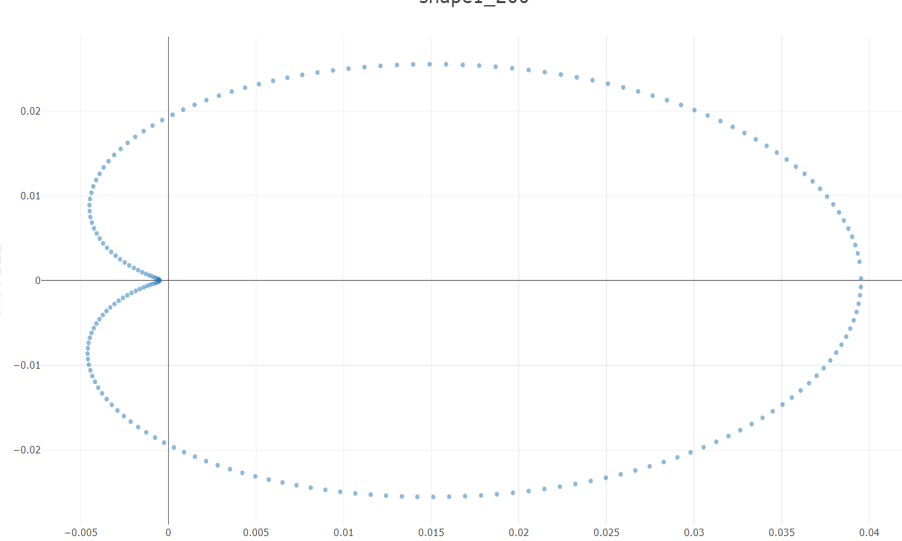
\includegraphics[width=\textwidth]{gfx/Read CSV Image.png}
	\caption{CSV Plot of a custom shape}
	\label{fig:validation:csv}
\end{figure}

The x and y coordinate values are read from a CSV file and the plot is as shown in Fig 5.1.
This plot will be rendered in the Ultrahaptics device. Fig 5.2 (a) represents the CSV plot being rendered on Ultrahaptics using AM technique and Fig 5.2 (b) represents the same CSV plot in TPS technique. 

\begin{figure}[H]
	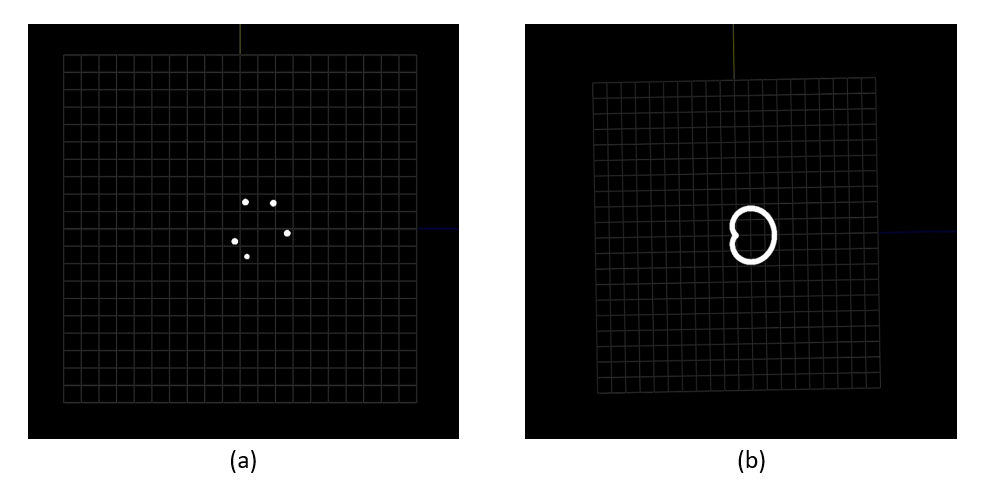
\includegraphics[width=\textwidth]{gfx/read_csv_rendering.png}
	\caption{(a) Ultraviz visualization of CSV plot in AM and (b) TPS technique}
	\label{fig:validation:csv_am}
\end{figure}

2. SVG file input feature:
\begin{figure}[H]
	\includegraphics[width=\textwidth]{gfx/SVG Input.png}
	\caption{SVG input shapes (a) Arrow Down (b) WiFi (c) Square}
	\label{fig:validation:svg}
\end{figure}

\begin{figure}[H]
	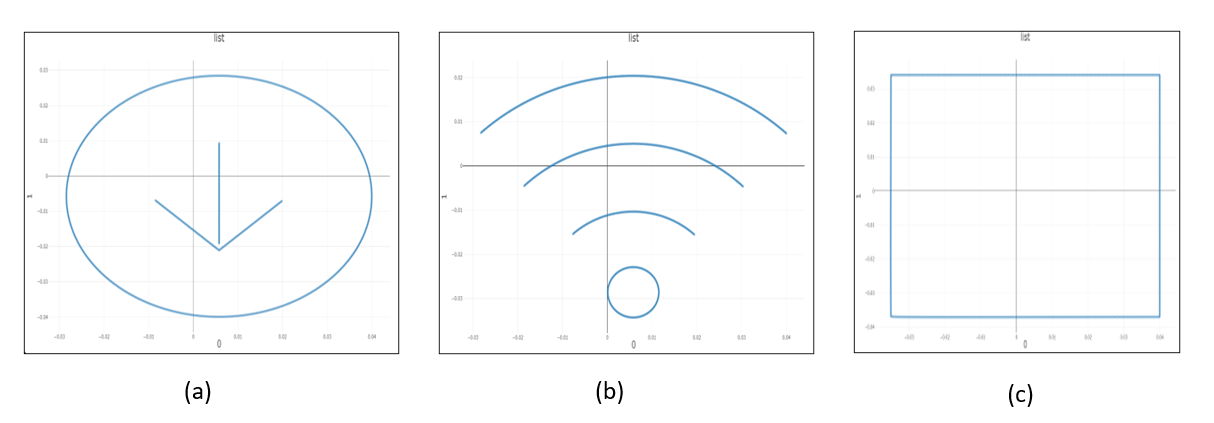
\includegraphics[width=\textwidth]{gfx/svg_plot.png}
	\caption{SVG plot of input shapes (a) Arrow Down (b) WiFi (c) Square}
	\label{fig:validation:svg_plot}
\end{figure}

Fig 5.3 depicts the various SVG files used to render on Ultrahaptics device. Once the SVG files are uploaded  it is converted to x and y coordinate system with specific number of points. Fig 5.4 shows the different xy plot of the SVG files uploaded.
 

\begin{figure}[H]
	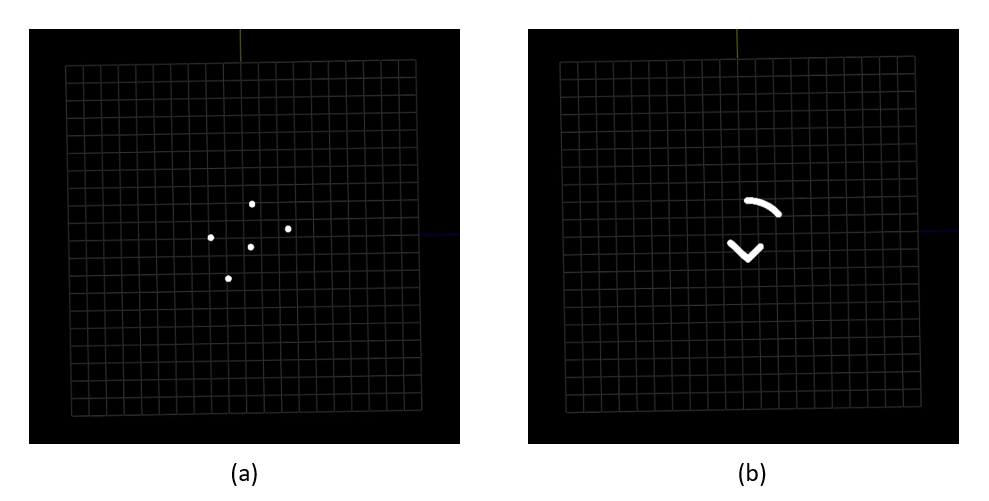
\includegraphics[width=\textwidth]{gfx/svg_ad.png}
	\caption{(a) SVG rendering of arrow down in AM (b) SVG rendering of arrow down in TPS}
	\label{fig:validation:svg_ad}
\end{figure}

\begin{figure}[H]
	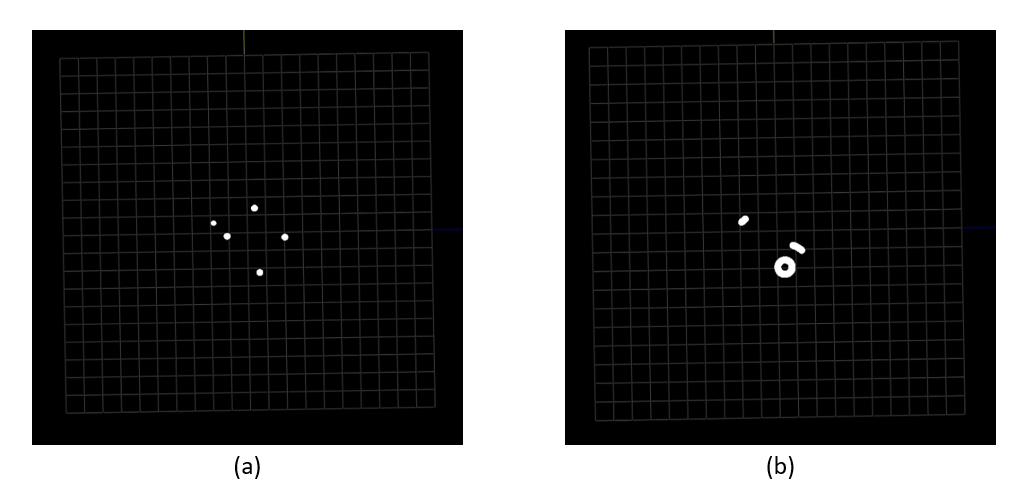
\includegraphics[width=\textwidth]{gfx/svg_wifi.png}
	\caption{(a) SVG rendering of WiFi in AM (b) SVG rendering of WiFi in TPS}
	\label{fig:validation:svg_wifi}
\end{figure}

\begin{figure}[H]
	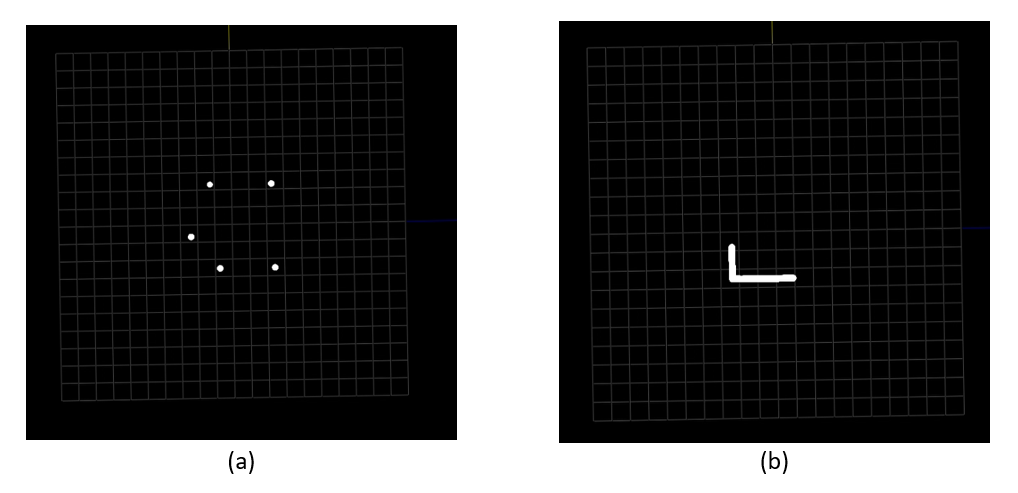
\includegraphics[width=\textwidth]{gfx/svg_sq.png}
	\caption{(a) SVG rendering of square in AM (b) SVG rendering of square in TPS}
	\label{fig:validation:svg_sq}
\end{figure}

Fig 5.5, Fig 5.6, Fig 5.7 displays an image of Ultraviz tool rendering the SVG inputs arrow down, WiFi and square in AM and TPS technique respectively.

3. Drawing on canvas:

The user can draw the shapes on the given HTML canvas using mouse. Fig 5.8 (a) shows a user drawn circle shape and Fig 5.8 (b) shows an plot of the user shape represented in x and y coordinate which will be eventually rendered on Ultrahatics.

\begin{figure}[H]
	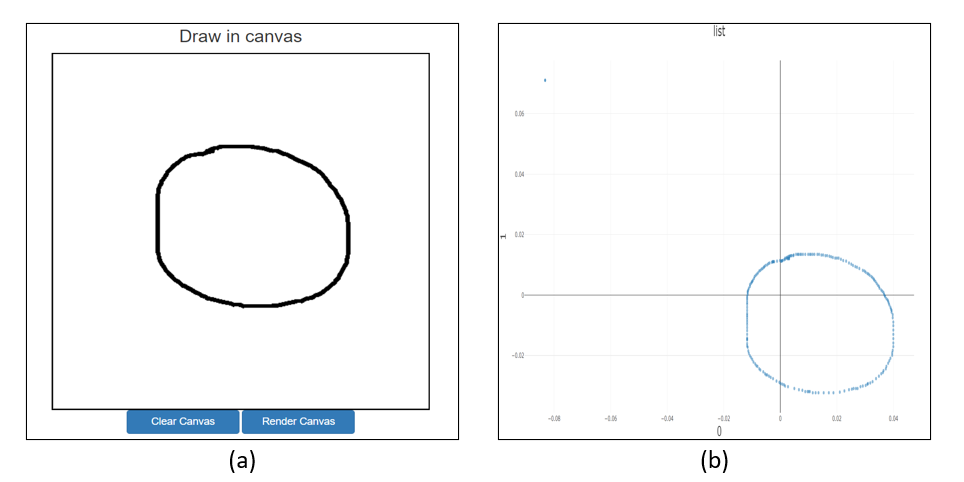
\includegraphics[width=\textwidth]{gfx/canvas input.png}
	\caption{(a) User drawn circle shape on HTML canvas (b) XY plot of the given user shape}
	\label{fig:validation:svg_sq_tps}
\end{figure}

Fig 5.9 (a) depicts the rendering of custom user shape in Ultraviz in AM and Fig 5.9 (b) depicts the same in TPS technique.

\begin{figure}[H]
	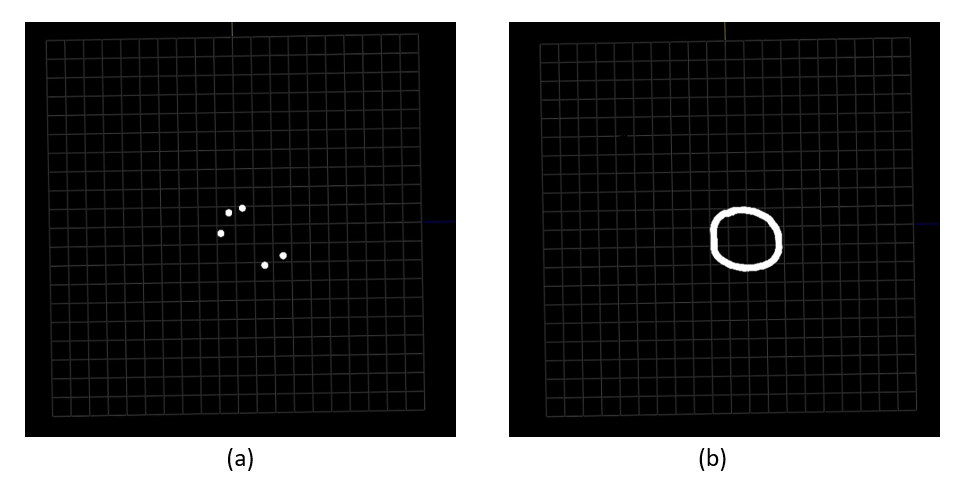
\includegraphics[width=\textwidth]{gfx/canvas_uv.png}
	\caption{(a) User drawn circle rendering in AM technique (b) User drawn circle rendering in TPS technique}
	\label{fig:validation:svg_sq_tps}
\end{figure}

4. Leap Canvas:

Leap canvas is similar to canvas drawing, instead of using mouse as a drawing tool here we use our index finger and with the help of Ultraleap leap motion device we draw on the canvas. Later the canvas drawing is converted to xy plot and then rendered on the Ultrahaptics device.

5. Leap Live:

Leap live uses the Ultraleap leap motion device to track our index finger and the same point is being rendered live on the Ultrahaptics device. The control point moves in the direction of the Ultraleap leap motion hand input.

\section{Cross validation and observation from developers}
\label{sec:validation:cross validation and observation from developers}

In order to further validate our project we conducted a short study between the authors of this project where we chose three different shapes i.e, square, circle and triangle and decided to guess the shape in various different techniques. In the first study we did not tell the observer on the Ultrahaptics which all shapes where there in the study and the observer guessed everything as circle. 

Later in the second study, we informed the observer the available shapes and then performed the study. We conducted the study mutually between us and below are the results:
Square shape was easily identified by both of us in AM technique and both guessed the square shape as circle in TPS technique. Triangle was guessed correctly in both the techniques. Circle was guessed correctly in TPS technique and one observer reported circle as triangle in AM technique. \\
Hence, from this short observation it was concluded that basic shapes if known to the subject in advance are recognized in a better manner.

Below in Fig 5.10 you can see all the results summed up in a table. 

\begin{figure}[H]
	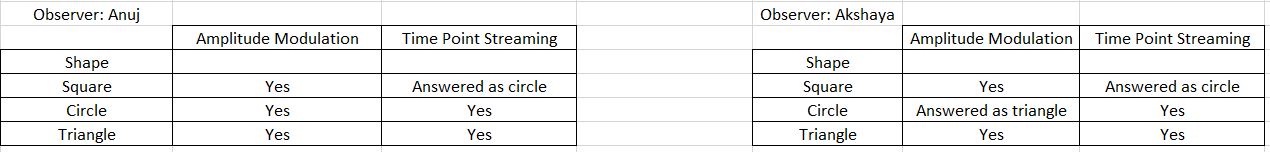
\includegraphics[width=150mm, height=25mm]{gfx/user_study_result.png}
	\caption{Results of validation between the authors of the project}
	\label{fig:validation:svg_sq_tps}
\end{figure}


\section{Oil bath}
\label{sec:validation:oilbath}

We also came across a technique where the rendering can be projected on an oil bath set-up to visualize how the inputs are being rendered on the user palm \cite{oil}. This experiment was a guided setup by the ultrahaptics support team. The step by step guide to set up the environment is as follows:

1. The Ultrahaptics device is suspended approximately 15cm above the oil bath using a robotic arm. There is no need to use the Leap Motion so the cradle can be separated. 

2. The oil is between 2 and 5mm deep. There is a purpose built perspex tank of 30 centimetres for the experiment. The oil must have the correct consistency and viscous enough to show dispersion, fluid enough to be responsive. We have found that a 50:50 mix of olive oil and pumpkin seed oil give good results. 

3. The oil bath must be raised approximately 3 cm above a white surface. We used legos for this purpose and used two A3 sheets of paper as a white surface.

4. Light with a single, small, bright light source from above or to an angle to project the shadow of the distorted surface on to the oil. There is a small, LED light available on an adjustable stalk. Place it between top of tank and perspex holder, with light covering as much of oil as possible. The light must be bright enough to reflect onto a wall and the room must be as dark as possible to achieve the best affect.

Fig 5.11 and Fig 5.12 show the experiment setup of oil bath. 

\begin{figure}[htb]
	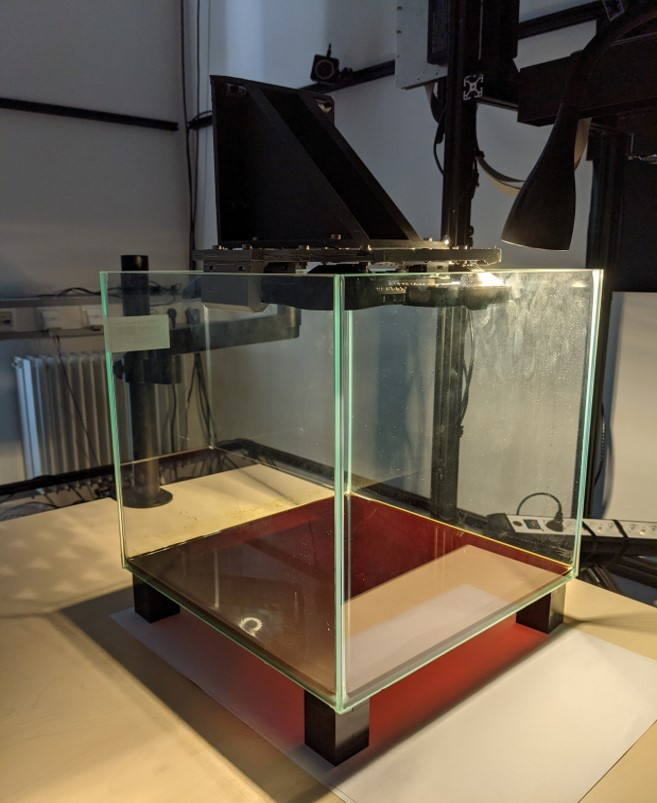
\includegraphics[width=\textwidth]{gfx/oilbath1.jpg}
	\caption{Overall oil bath setup}
	\label{fig:validation:oil_bath1}
\end{figure}

\begin{figure}[htb]
	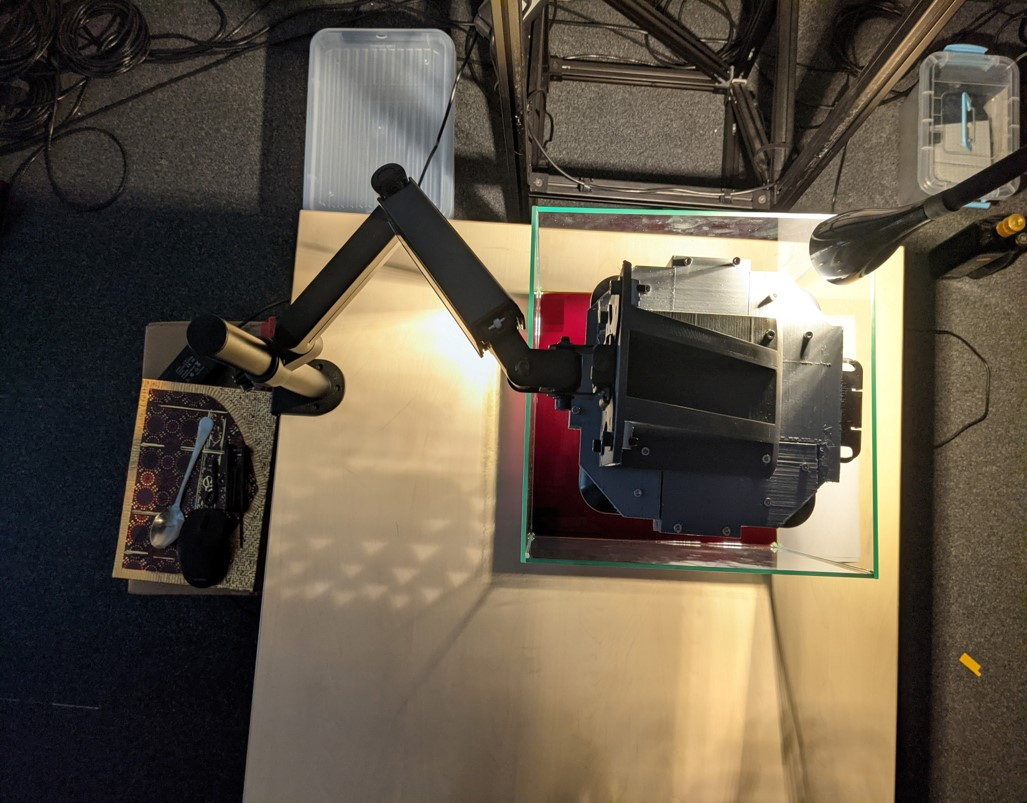
\includegraphics[width=\textwidth]{gfx/oilbath2.jpg}
	\caption{Top view of oil bath setup }
	\label{fig:validation:oil_bath2}
\end{figure}